\section{Implementierung mit Xamarin}
In diesem Abschnitt wird die Implementierung der N��ing ScanApp mit Xamarin.Forms beschrieben. 
\subsection{Architekturmuster}
F�r die Entwicklung der Applikation wurde das f�r Xamarin �bliche MVVM-Muster angewendet.
\subsection{Persistierung der Daten}
F�r die Persistenz der Appdaten wurde SQLite eingesetzt.
\subsection{Views}
Xamarin l�sst Entwicklern die Wahl zwischen der Markupsprache Xaml und C\# f�r die Implementierung
der Benutzeroberfl�chen. Mit C\# lassen sich die Positionierung der Steuerelemente und deren
Funktionalit�t in einer C\#-Datei implementieren, aber das macht den Code schwer lesbar und nicht
wiederverwendbar. Aus diesem Grund wurden die grafischen Interfaces der N��ing ScanApp mit der
Markupsprache Xaml beschrieben.
Somit wurde eine strikte Trennung zwischen dem Oberfl�chendesign (in einer
Xaml-Datei beschrieben) und der Funktionalit�t (in der
zugrundeliegenden (Code-Behind) C\#-Datei implementiert) erreicht. Ein weiterer Vorteil von der
Benutzung von Xaml ist die daraus entstehende M�glichkeit, dass Designer und Entwickler unabh�ngig
voneinander arbeiten k�nnen.\\Bei der Erstellung einer Xamarin.Forms ContentPage Xaml-Datei wird
automatisch auch die zugrundeliegende C\#-Datei angelegt (siehe Abb. \ref{fig:abb21}).

 In Abbildung \ref{fig:abb23} sieht man den Xaml-Code f�r die Benutzeroberfl�che, die in Abbildung
\ref{fig:abb24} zu sehen ist. Der Aufbau einer Xaml-Datei entspricht eines XML-Dokuments. Es gibt ein Wurzelelement und jedes
Element kann Attribute besitzen. Dadurch entsteht eine �bersichtliche Hierarchie der Elemente. Durch
das Attribut x:Name kann man auf das Element aus dem Code-Behind-Datei zugreifen und so kann man
z.B. den Text eines Labels oder die Textfarbe �ndern (siehe \ref{fig:abb26}).
\\In Abbildung \ref{fig:abb25} sieht man die zugrundeliegenden C\#-Datei, in der z.B. die
Funktionalit�t der Toolbar-Buttons implementiert ist. Beim Klick auf den Button zum Speichern der
Angaben, werden die Texten der Texteingabefeldern in einem Objekt vom Typ Kopfdaten gespeichert und
anschlie�end wird das neu erstellte Objekt in die SQLite-Datenbank gespeichert. Beim Klick auf den
M�llkorb-Button, werden die gespeicherten pers�nlichen Daten aus der SQLite-Datenbank gel�scht. 
\begin{figure}[!h]
\centering

\includegraphics[scale = 0.7]{graphics/XamlDateiPlusCSDatei.png}
\caption{Xaml-Datei und die zugrundeliegende C\#-Datei}
\label{fig:abb21}
\end{figure}

\begin{figure}[!h]
\centering
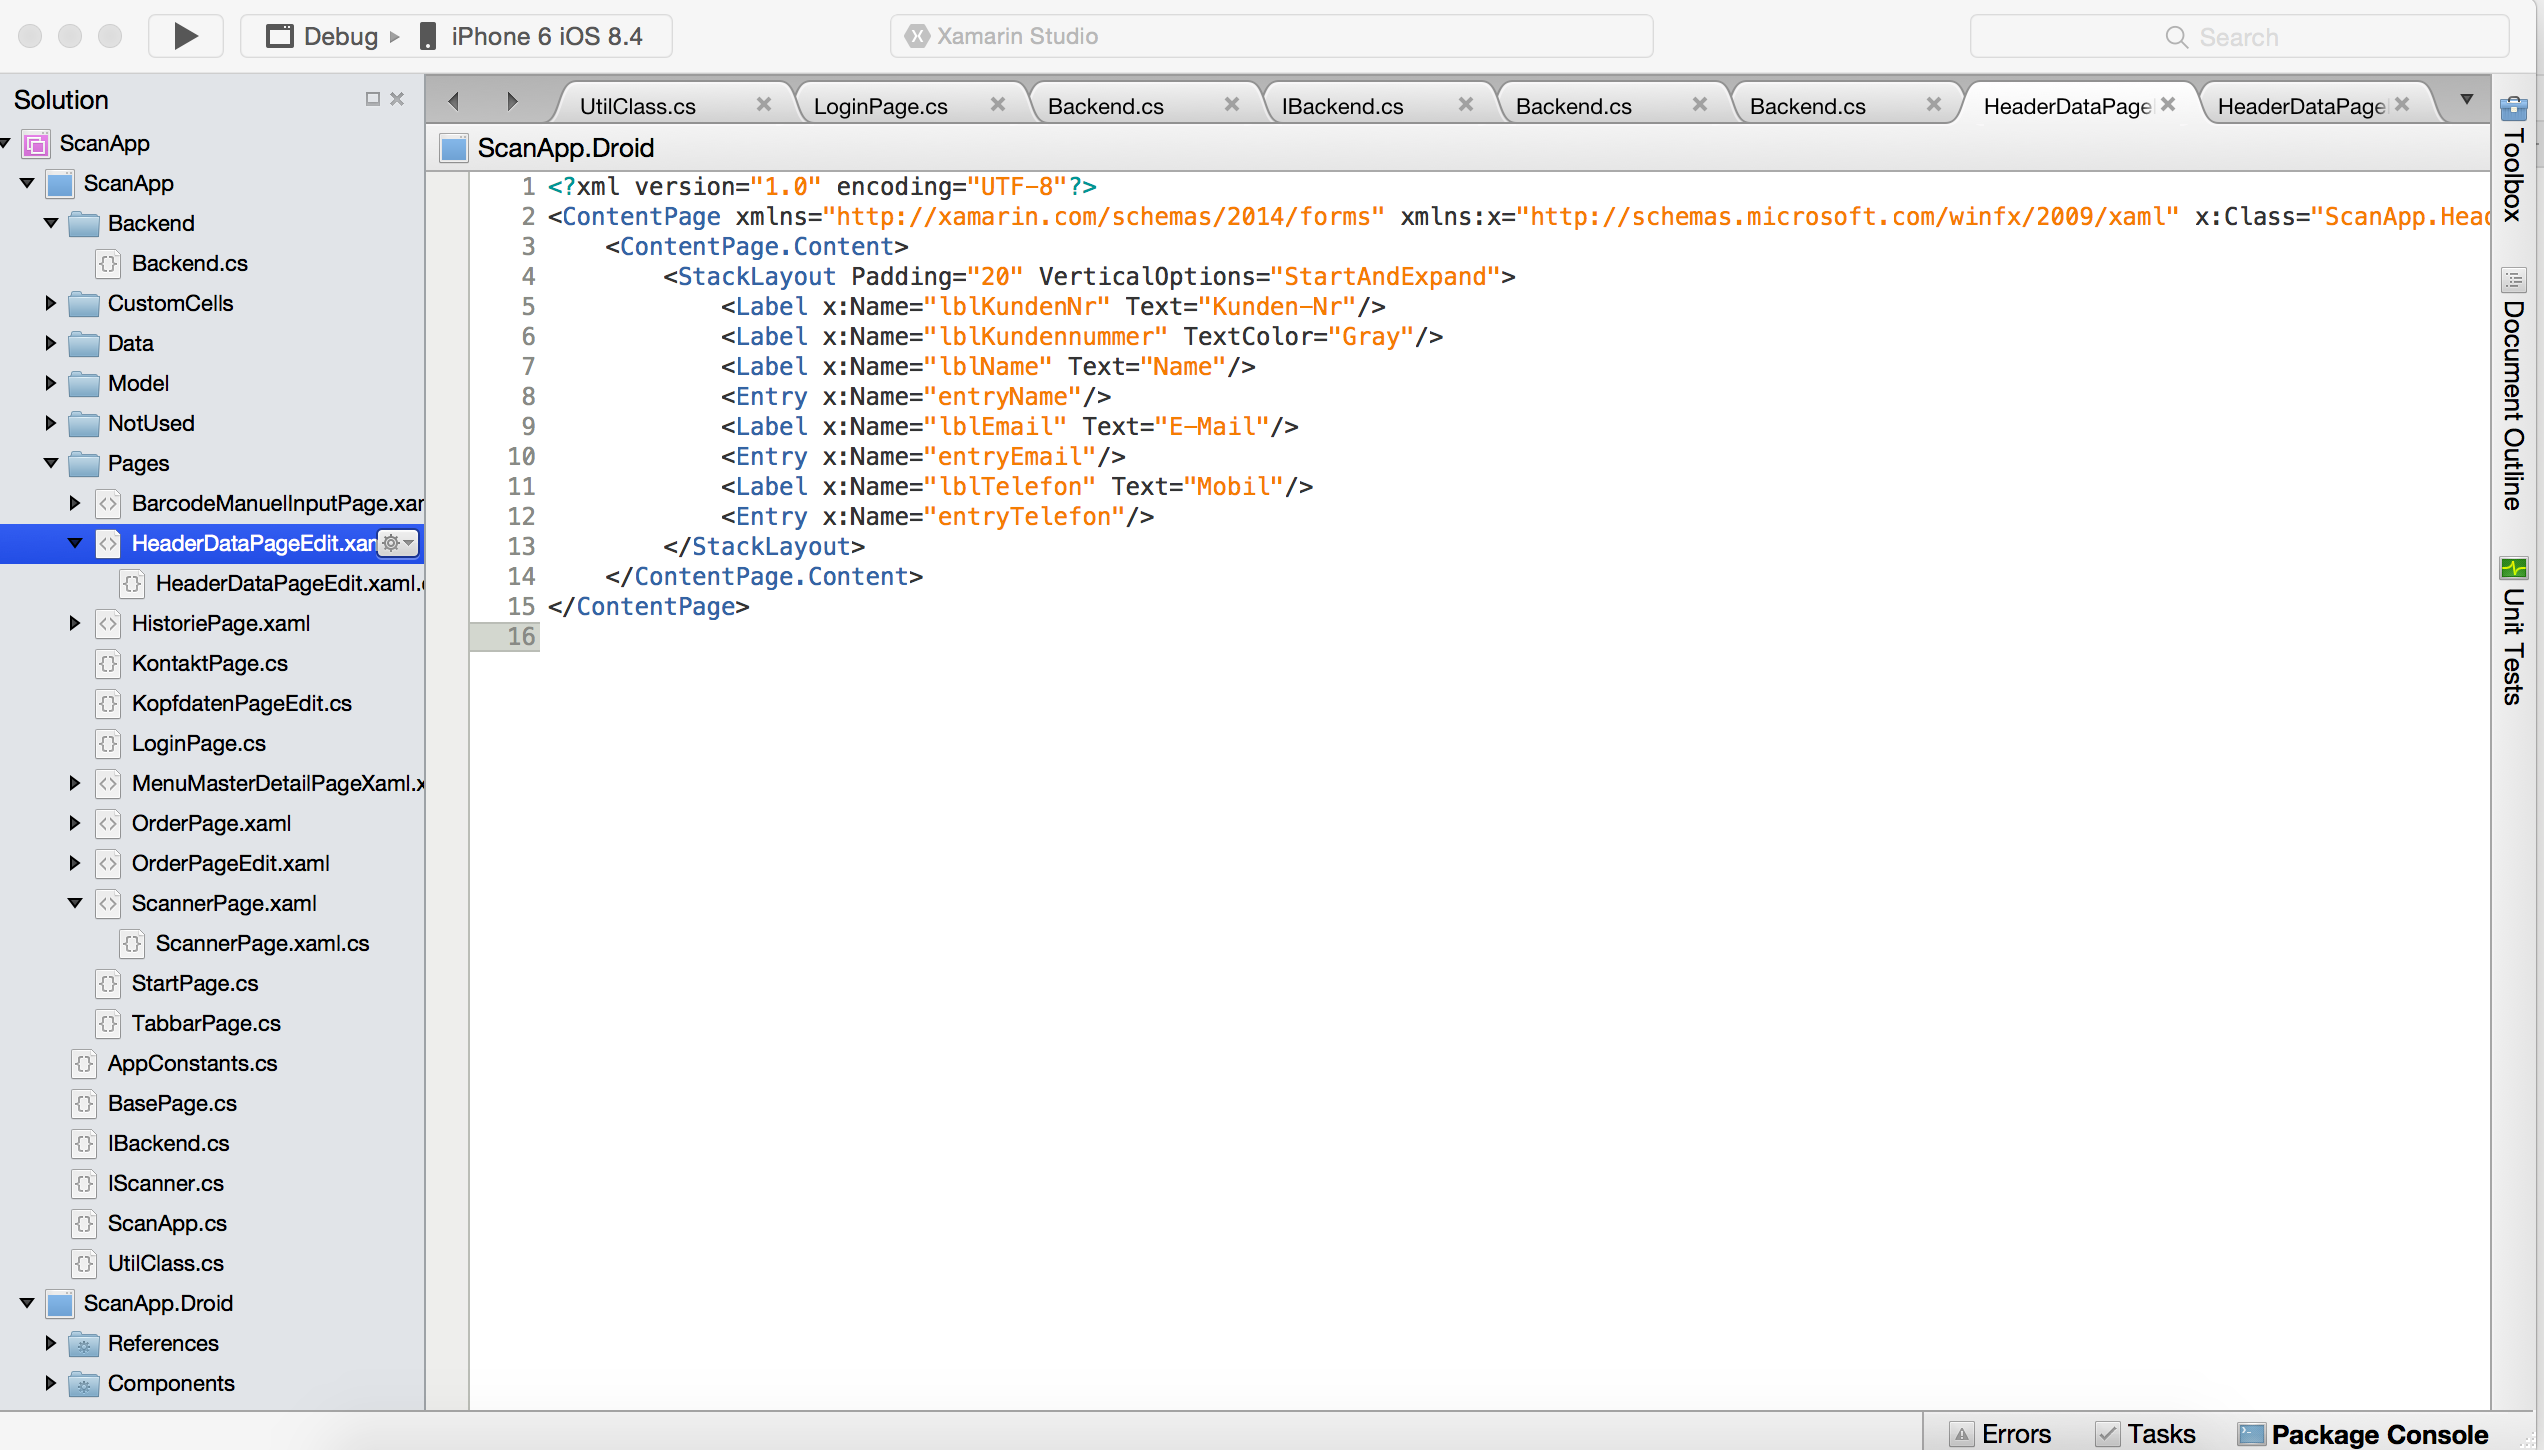
\includegraphics[scale = 0.324]{graphics/XamlDatei.png}
\caption{Xaml-Datei}
\label{fig:abb23}
\end{figure}
\begin{figure}[!h]
\centering
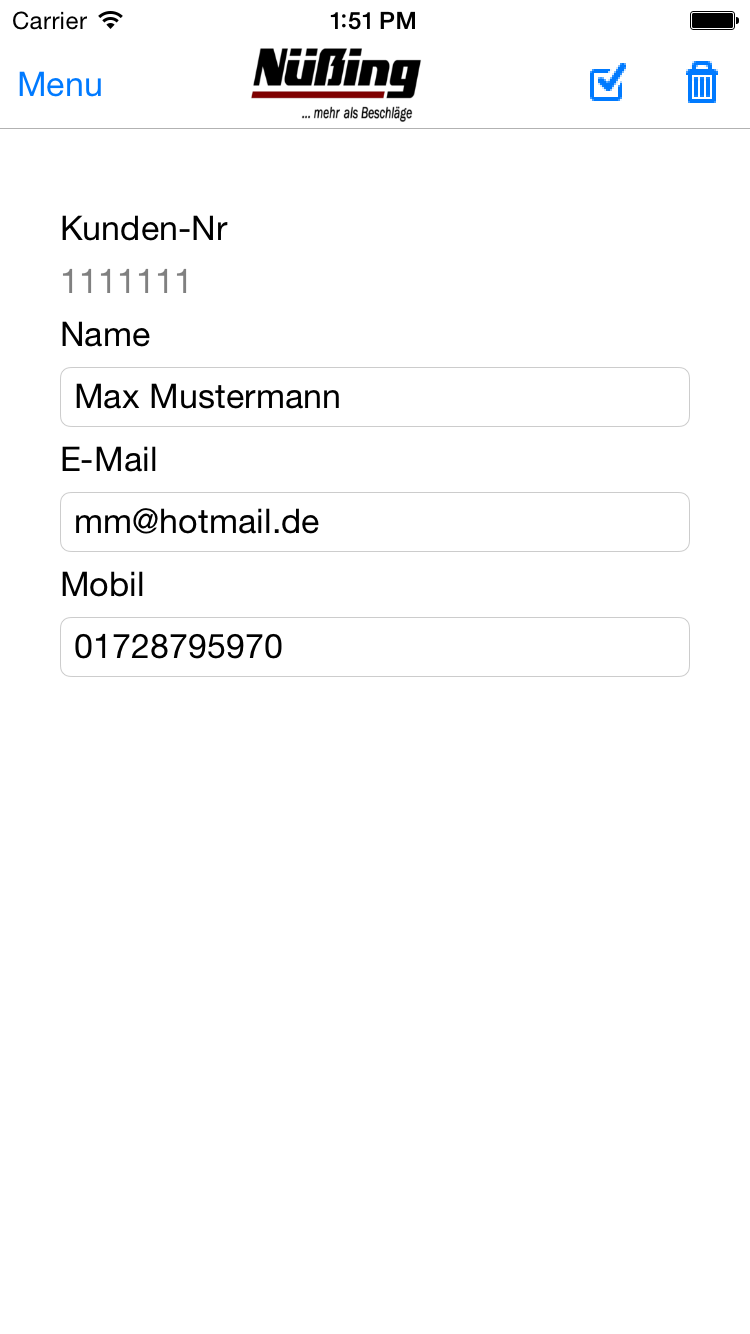
\includegraphics[scale = 0.3]{graphics/appScreenshots/PersoenlicheDaten.png}
\caption{Seite zum Editieren der pers�nlichen Daten eines Nutzers der ScanApp}
\label{fig:abb24}
\end{figure}
\begin{figure}[!h]
\centering
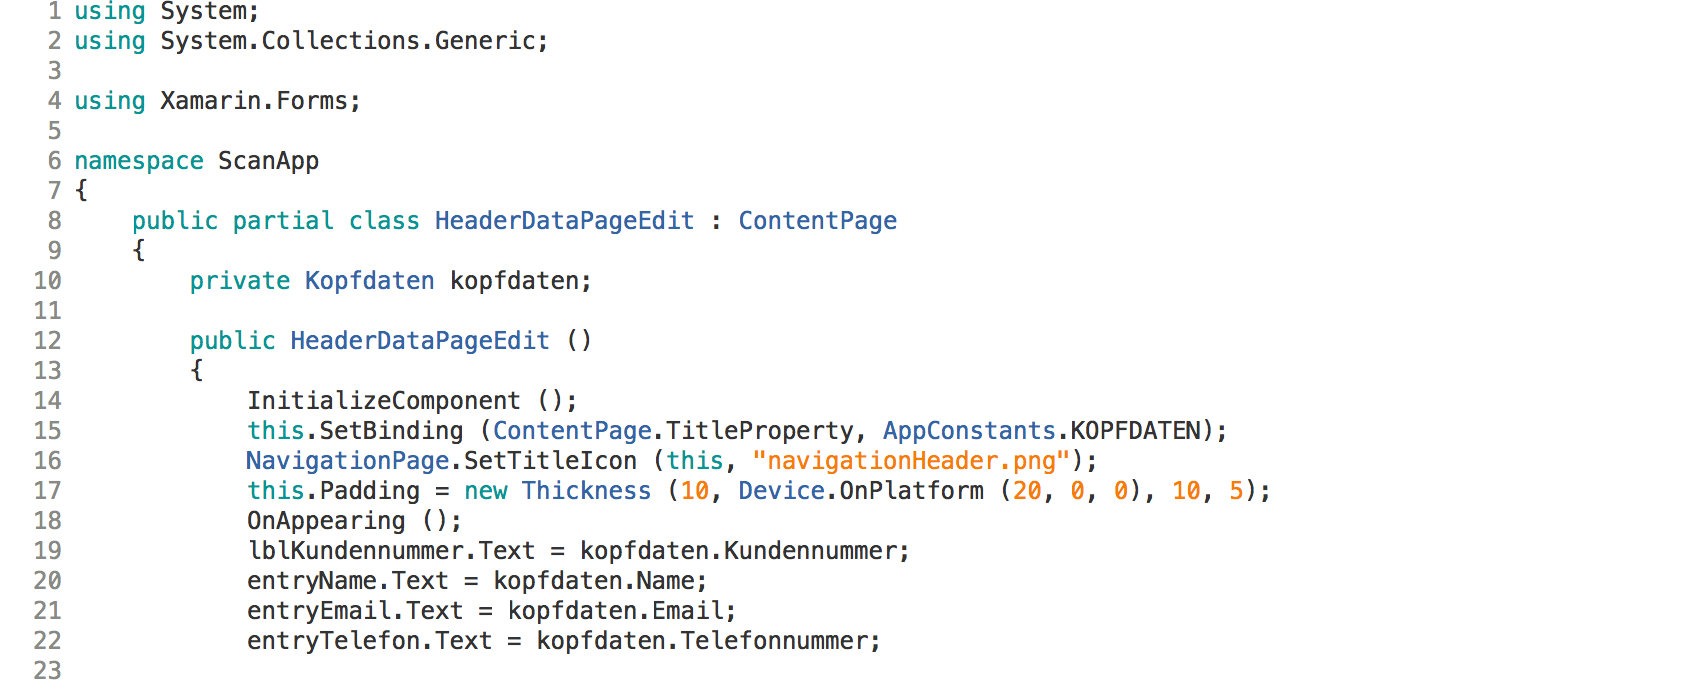
\includegraphics[scale = 0.5]{graphics/HeaderDatenCSDatei.png}
\caption{Zugrundeliegende (Code-Behind) C\#-Datei}
\label{fig:abb26}
\end{figure}
\begin{figure}[!h]
\centering
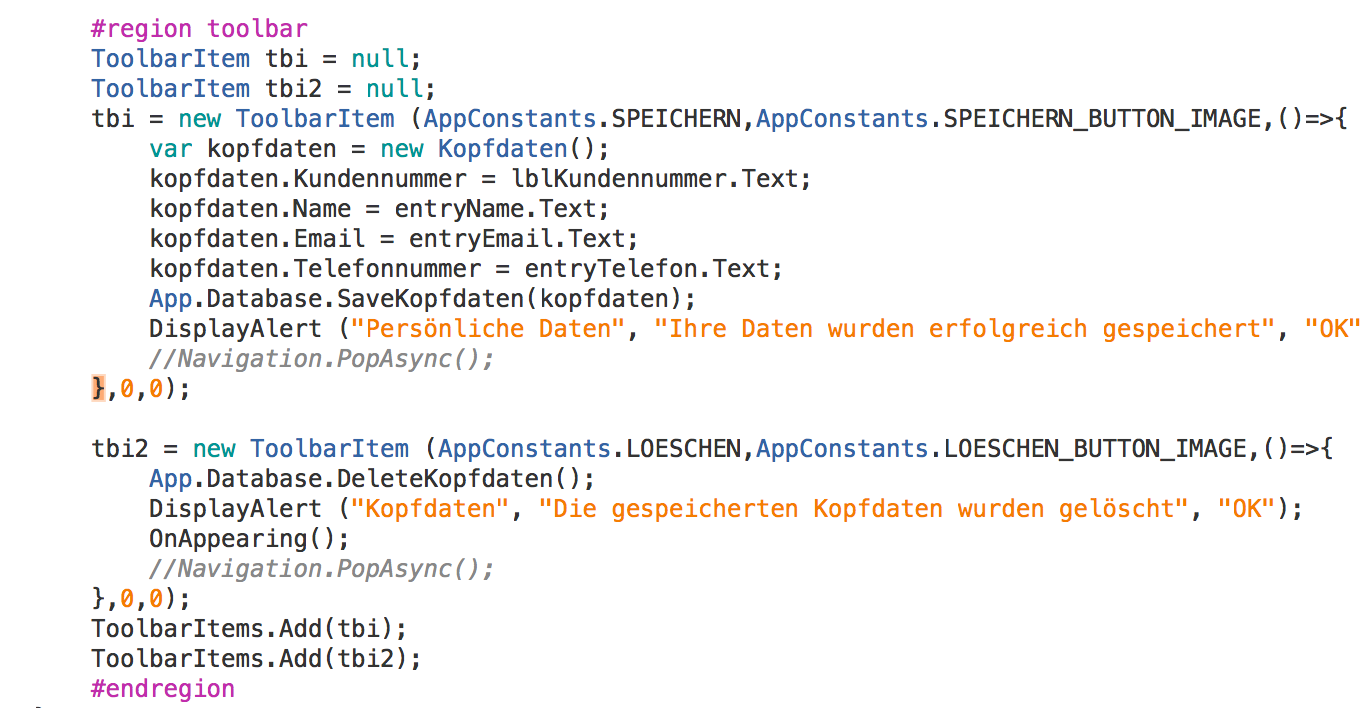
\includegraphics[scale = 0.5]{graphics/HeaderDatenToolbar.png}
\caption{Zugrundeliegende C\#-Datei}
\label{fig:abb25}
\end{figure}